\chapter{System components}

This chapter provides a comprehensive examination of the electronic components and systems integrated into the MMU system. It begins with a key decision made independently—the selection of the microcontroller. Further, this the chapter introduces choices made by the electronics team, detailing the roles and specifications of other components such as DC motors, motor drivers, and Hall effect sensors. These components ensure precise operation and control within the MMU. Through technical descriptions and schematic overviews, the chapter not only highlights the functionalities of these components but also illustrates their integration and interaction within the MMU system.

\section{Microcontroller}

\subsection{Microcontroller analysis}

When considering microcontrollers for MMU project, the choices from Texas Instruments, STMicroelectronics, and AVR each come with their distinct advantages and typical usage scenarios.

Texas Instruments microcontrollers are known for their low power consumption, which makes them suitable for battery-operated devices like portable health monitors and smart sensors. They feature advanced power management capabilities that help extend their operational lifetime in energy-sensitive applications. Additionally, Texas Instruments provides a wide array of microcontroller options that support various wireless communication protocols.

STMicroelectronics, particularly the STM32 series used in the MK4 printer, is preferred for its high performance and broad range of features. These microcontrollers provide powerful processing capabilities and flexible connectivity options, including USB, Ethernet, and Bluetooth. They are ideal for complex applications such as multimedia processing and IoT devices that handle various data types. However, these microcontrollers generally have higher power consumption, which may not be suitable for the most power-sensitive projects.

AVR microcontrollers, currently used in the MMU, are noted for their simplicity and ease of use. They are particularly well-suited for rapid prototyping and small-scale projects thanks to easy programming and integration. While their performance adequately meets the needs of many applications, such as simple robotics and home automation systems, they may lack the necessary processing power for more demanding tasks. Compared to Texas Instruments and STM, AVR microcontrollers may offer fewer resources and less advanced peripherals.

In summary, the selected microcontroller for this project is the MSPM0G3507 from Texas Instrumentso \cite{mspm0g3507}. The MSPM0G3507 provides performance comparable to the STM32 but at a lower cost than AVR, making it a compelling choice \cite{avr-price}.

\subsection{MSPM0G3507}

The MSPM0G3507 microcontroller is a highly integrated, ultra-low-power device designed for a range of applications from motor control to factory automation. Based on the Arm Cortex-M0+ core \cite{arm-cortex} operating at up to 80 MHz, it features robust digital and analog capabilities. This includes up to 128KB of flash memory with error correction and up to 32KB of SRAM with hardware parity. Its analog capabilities are substantial, with multiple high-speed ADCs and DACs, comparators, and zero-drift amplifiers, which make it suitable for precise measurement and control tasks.

The microcontroller also supports a range of communication protocols including multiple UART interfaces, I2C, SPI, and CAN-FD, making it versatile for different communication needs. It is built to operate in a wide range of environmental conditions, supporting temperatures from -40°C to 125°C and a voltage range from 1.62V to 3.6V.

For power management, it offers several low-power modes that significantly reduce energy consumption when idle or in standby, which is essential for battery-operated devices. The device includes advanced security features such as AES encryption and a true random number generator, ensuring data integrity and security in sensitive applications \cite{mspm0-manual}.

\section{Direct current motor}

In MMU, DC motors are used to manage the filament selection process. Each filament type is loaded into a separate channel within the MMU, and the DC motor is responsible for driving the selected filament towards the extruder. This system allows for switching between different filaments during a single print job.

In the Figure~\ref{fig:dc_motor_ic}, on the left there is an X-ray image of an integrated circuit, showcasing the internal components of a motor. The X-ray gives us a clear view of the layout and structure within the device. On the right side, there is a neatly organized schematic diagram. This serves as a visual guide to the motor's circuitry, detailing the connections and components. Together, these two elements offer a comprehensive overview of the motor's design.

\begin{figure}[H]
    \centering
    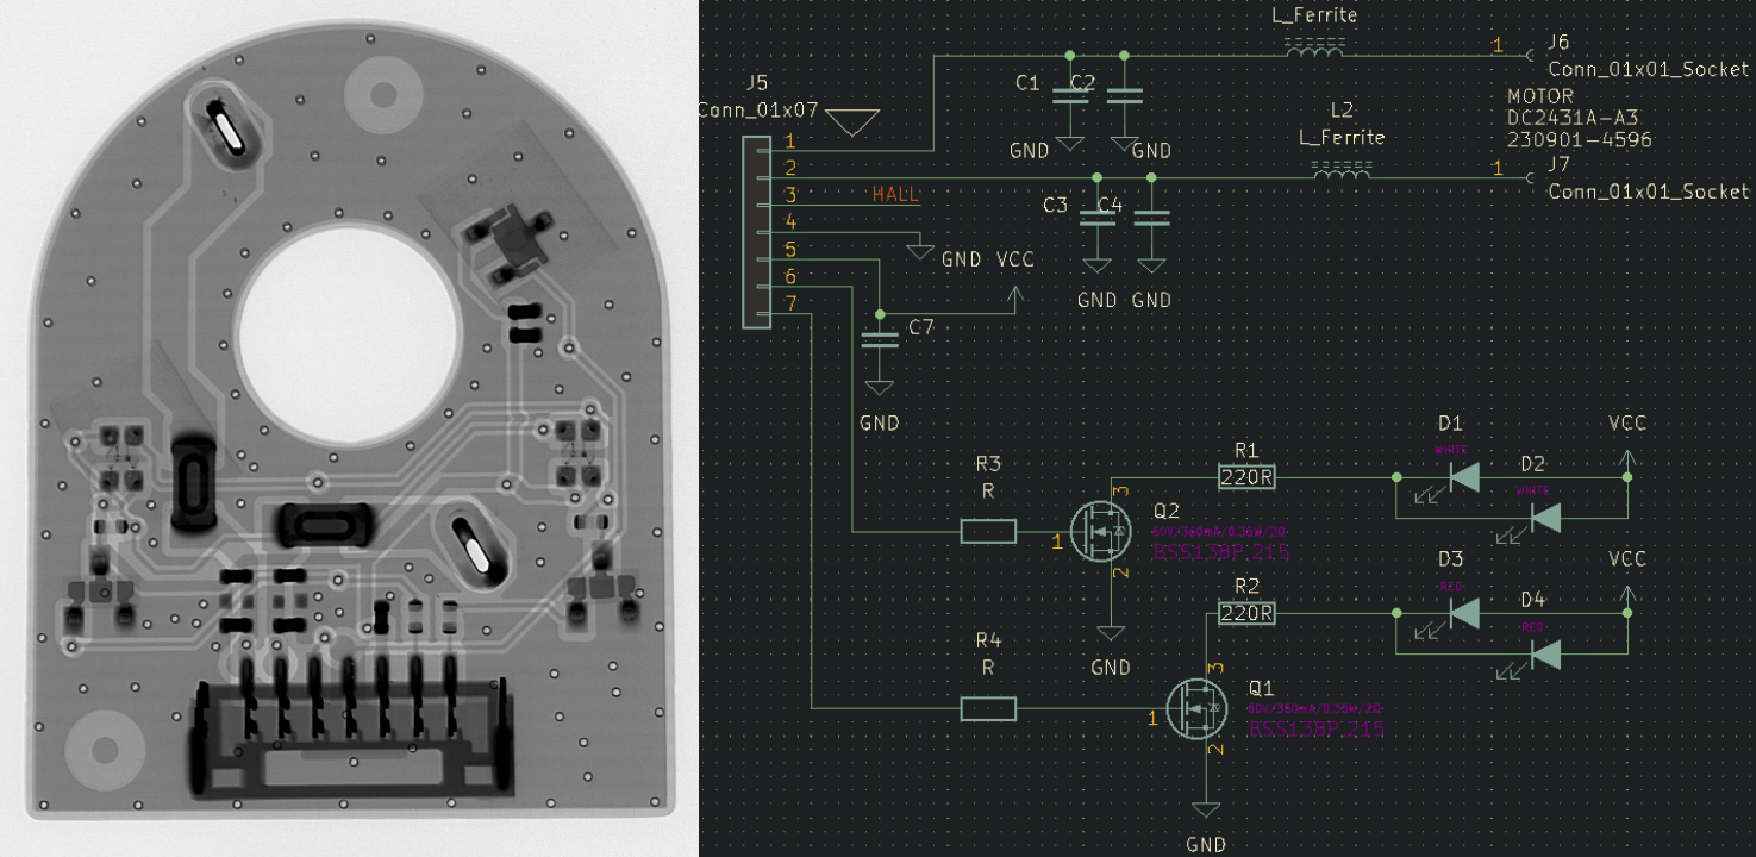
\includegraphics[width=0.8\linewidth]{img/dc_motor}
    \caption{DC motor}
    \label{fig:dc_motor_ic} 
\end{figure}

\section{Direct current motor driver}

The Pololu TB6612FNG Dual Motor Driver Carrier \cite{motor-driver} is a compact module that allows for control of two bidirectional DC motors or one bipolar stepper motor. It utilizes Toshiba's TB6612FNG motor driver integrated circuit. The board supports a motor voltage range of 4.5V to 13.5V and can deliver up to 3A per channel in peak output with a continuous current of 1A per channel, which can be increased to 2A if channels are paralleled. The logic voltage can be between 2.7V and 5.5V. It includes built-in thermal shutdown, filtering capacitors on both supply lines, and reverse-power protection on the motor supply.

\section{Hall effect sensor}

A Hall effect sensor is a type of magnetic sensor, which when exposed to a magnetic field perpendicular to the current's flow in a conductor, a voltage—known as Hall voltage—is generated across the conductor. This voltage is perpendicular to both the current and the magnetic field, allowing the sensor to detect the strength and changes in the magnetic field.

In this project, the MT9105 variant \cite{hall-effect-sensor} from the MT910X series of linear Hall effect is utilized. The MT9105 operates within a 3.0V to 5.5V voltage range and outputs a voltage at half of the supply voltage when no magnetic field is present. The sensor's output varies linearly with the magnetic flux density, offering different sensitivity settings to maximize output voltage swing based on the required sensing range. It also responds distinctly to the north and south poles of a magnet.

\section{Filament Hub}

The role of the Filament Hub is to keep the PTFE tubes, corresponding to each slot of the MMU, organized and held together, thus ensuring smooth feeding of the filament to the extruder.

On the circuit board, in Figure~\ref{fig:hub_ic}, three MT9105 Hall sensors are installed, each serving a different function. The filament sensor connector includes duplicate power supply pins and three analog outputs corresponding to these sensors. The first output is connected to a Hall sensor that detects the presence of filament in the extruder. The second output is linked to another Hall sensor that monitors the cutting blade's interaction with the filament; however, there is currently no implemented solution for cutting, making this sensor non-functional for its intended purpose. The third output measures the tension of the filament in the Bowden tube.

\begin{figure}[H]
    \centering
    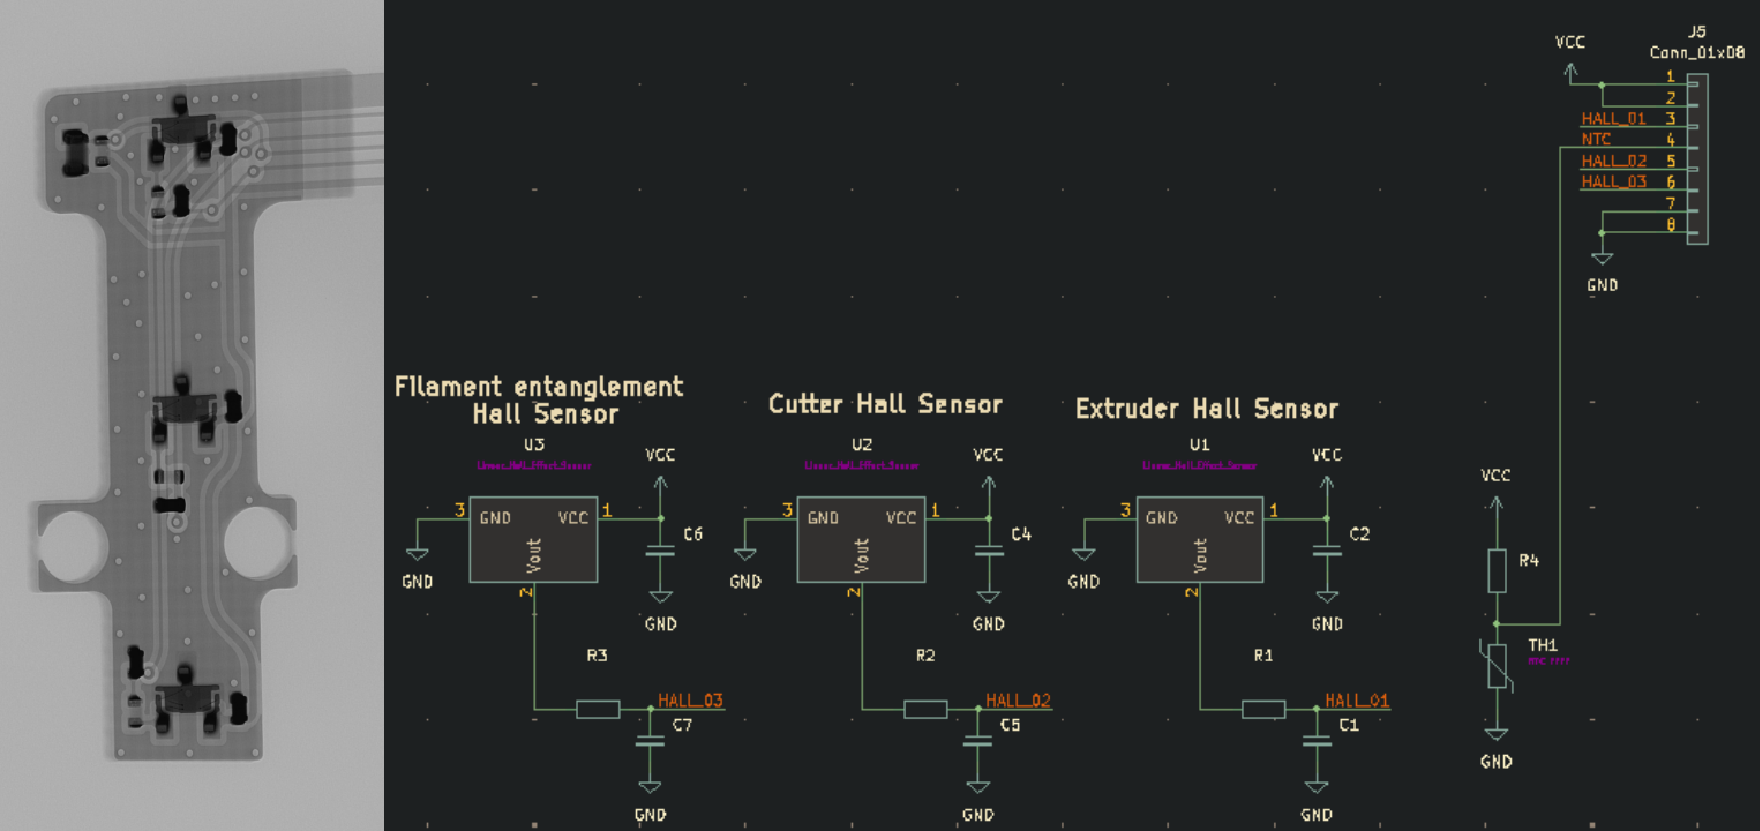
\includegraphics[width=0.8\linewidth]{img/filament_hub}
    \caption{Filament Hub}
    \label{fig:hub_ic} 
\end{figure}

\section{Filament sensor in feeding system}

The filament sensor in MMU feeding system acts as a guard and ensures smooth passage of filament from the spool to the printer's extruder. The sensor's main function is to detect the presence of filament and alerts the system to any shortage or breakage that could interrupt printing. This early detection allows the printer to pause and offers the user an option to rectify the issue without compromising the print job.

By monitoring the movement and flow of the filament, the sensor helps the printer adjust the pull from the spool in real-time, reducing the risk of knots or obstructions that could lead to print failure. Furthermore, the filament sensor facilitates automated loading and unloading of filament.

The Figure~\ref{fig:fsensor_ic} displays an X-ray image of an integrated circuit of filament sensor in the feeding system.

\begin{figure}[H]
    \centering
    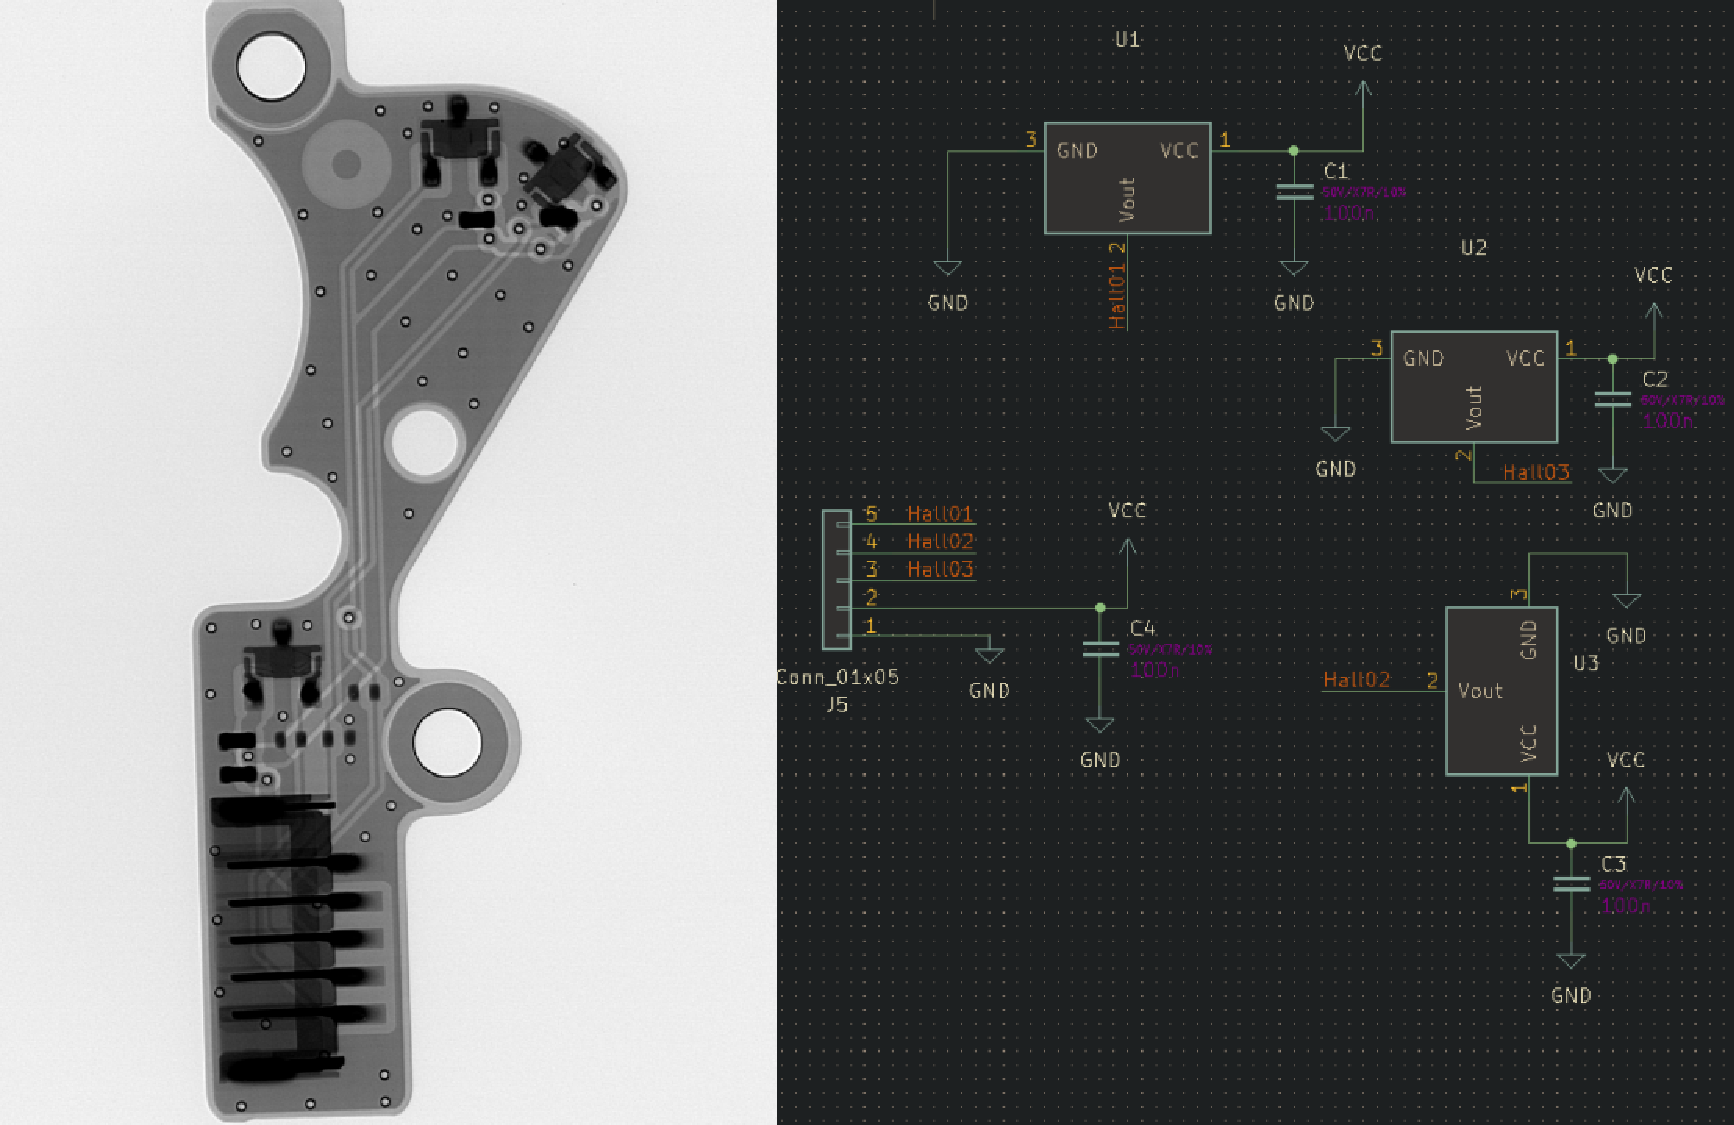
\includegraphics[width=0.8\linewidth]{img/filament_sensor}
    \caption{Filament sensor}
    \label{fig:fsensor_ic} 
\end{figure}
